% Options for packages loaded elsewhere
\PassOptionsToPackage{unicode}{hyperref}
\PassOptionsToPackage{hyphens}{url}
\PassOptionsToPackage{dvipsnames,svgnames,x11names}{xcolor}
%
\documentclass[
  letterpaper,
  DIV=11,
  numbers=noendperiod]{scrreprt}

\usepackage{amsmath,amssymb}
\usepackage{iftex}
\ifPDFTeX
  \usepackage[T1]{fontenc}
  \usepackage[utf8]{inputenc}
  \usepackage{textcomp} % provide euro and other symbols
\else % if luatex or xetex
  \usepackage{unicode-math}
  \defaultfontfeatures{Scale=MatchLowercase}
  \defaultfontfeatures[\rmfamily]{Ligatures=TeX,Scale=1}
\fi
\usepackage{lmodern}
\ifPDFTeX\else  
    % xetex/luatex font selection
\fi
% Use upquote if available, for straight quotes in verbatim environments
\IfFileExists{upquote.sty}{\usepackage{upquote}}{}
\IfFileExists{microtype.sty}{% use microtype if available
  \usepackage[]{microtype}
  \UseMicrotypeSet[protrusion]{basicmath} % disable protrusion for tt fonts
}{}
\makeatletter
\@ifundefined{KOMAClassName}{% if non-KOMA class
  \IfFileExists{parskip.sty}{%
    \usepackage{parskip}
  }{% else
    \setlength{\parindent}{0pt}
    \setlength{\parskip}{6pt plus 2pt minus 1pt}}
}{% if KOMA class
  \KOMAoptions{parskip=half}}
\makeatother
\usepackage{xcolor}
\setlength{\emergencystretch}{3em} % prevent overfull lines
\setcounter{secnumdepth}{5}
% Make \paragraph and \subparagraph free-standing
\makeatletter
\ifx\paragraph\undefined\else
  \let\oldparagraph\paragraph
  \renewcommand{\paragraph}{
    \@ifstar
      \xxxParagraphStar
      \xxxParagraphNoStar
  }
  \newcommand{\xxxParagraphStar}[1]{\oldparagraph*{#1}\mbox{}}
  \newcommand{\xxxParagraphNoStar}[1]{\oldparagraph{#1}\mbox{}}
\fi
\ifx\subparagraph\undefined\else
  \let\oldsubparagraph\subparagraph
  \renewcommand{\subparagraph}{
    \@ifstar
      \xxxSubParagraphStar
      \xxxSubParagraphNoStar
  }
  \newcommand{\xxxSubParagraphStar}[1]{\oldsubparagraph*{#1}\mbox{}}
  \newcommand{\xxxSubParagraphNoStar}[1]{\oldsubparagraph{#1}\mbox{}}
\fi
\makeatother

\usepackage{color}
\usepackage{fancyvrb}
\newcommand{\VerbBar}{|}
\newcommand{\VERB}{\Verb[commandchars=\\\{\}]}
\DefineVerbatimEnvironment{Highlighting}{Verbatim}{commandchars=\\\{\}}
% Add ',fontsize=\small' for more characters per line
\usepackage{framed}
\definecolor{shadecolor}{RGB}{241,243,245}
\newenvironment{Shaded}{\begin{snugshade}}{\end{snugshade}}
\newcommand{\AlertTok}[1]{\textcolor[rgb]{0.68,0.00,0.00}{#1}}
\newcommand{\AnnotationTok}[1]{\textcolor[rgb]{0.37,0.37,0.37}{#1}}
\newcommand{\AttributeTok}[1]{\textcolor[rgb]{0.40,0.45,0.13}{#1}}
\newcommand{\BaseNTok}[1]{\textcolor[rgb]{0.68,0.00,0.00}{#1}}
\newcommand{\BuiltInTok}[1]{\textcolor[rgb]{0.00,0.23,0.31}{#1}}
\newcommand{\CharTok}[1]{\textcolor[rgb]{0.13,0.47,0.30}{#1}}
\newcommand{\CommentTok}[1]{\textcolor[rgb]{0.37,0.37,0.37}{#1}}
\newcommand{\CommentVarTok}[1]{\textcolor[rgb]{0.37,0.37,0.37}{\textit{#1}}}
\newcommand{\ConstantTok}[1]{\textcolor[rgb]{0.56,0.35,0.01}{#1}}
\newcommand{\ControlFlowTok}[1]{\textcolor[rgb]{0.00,0.23,0.31}{\textbf{#1}}}
\newcommand{\DataTypeTok}[1]{\textcolor[rgb]{0.68,0.00,0.00}{#1}}
\newcommand{\DecValTok}[1]{\textcolor[rgb]{0.68,0.00,0.00}{#1}}
\newcommand{\DocumentationTok}[1]{\textcolor[rgb]{0.37,0.37,0.37}{\textit{#1}}}
\newcommand{\ErrorTok}[1]{\textcolor[rgb]{0.68,0.00,0.00}{#1}}
\newcommand{\ExtensionTok}[1]{\textcolor[rgb]{0.00,0.23,0.31}{#1}}
\newcommand{\FloatTok}[1]{\textcolor[rgb]{0.68,0.00,0.00}{#1}}
\newcommand{\FunctionTok}[1]{\textcolor[rgb]{0.28,0.35,0.67}{#1}}
\newcommand{\ImportTok}[1]{\textcolor[rgb]{0.00,0.46,0.62}{#1}}
\newcommand{\InformationTok}[1]{\textcolor[rgb]{0.37,0.37,0.37}{#1}}
\newcommand{\KeywordTok}[1]{\textcolor[rgb]{0.00,0.23,0.31}{\textbf{#1}}}
\newcommand{\NormalTok}[1]{\textcolor[rgb]{0.00,0.23,0.31}{#1}}
\newcommand{\OperatorTok}[1]{\textcolor[rgb]{0.37,0.37,0.37}{#1}}
\newcommand{\OtherTok}[1]{\textcolor[rgb]{0.00,0.23,0.31}{#1}}
\newcommand{\PreprocessorTok}[1]{\textcolor[rgb]{0.68,0.00,0.00}{#1}}
\newcommand{\RegionMarkerTok}[1]{\textcolor[rgb]{0.00,0.23,0.31}{#1}}
\newcommand{\SpecialCharTok}[1]{\textcolor[rgb]{0.37,0.37,0.37}{#1}}
\newcommand{\SpecialStringTok}[1]{\textcolor[rgb]{0.13,0.47,0.30}{#1}}
\newcommand{\StringTok}[1]{\textcolor[rgb]{0.13,0.47,0.30}{#1}}
\newcommand{\VariableTok}[1]{\textcolor[rgb]{0.07,0.07,0.07}{#1}}
\newcommand{\VerbatimStringTok}[1]{\textcolor[rgb]{0.13,0.47,0.30}{#1}}
\newcommand{\WarningTok}[1]{\textcolor[rgb]{0.37,0.37,0.37}{\textit{#1}}}

\providecommand{\tightlist}{%
  \setlength{\itemsep}{0pt}\setlength{\parskip}{0pt}}\usepackage{longtable,booktabs,array}
\usepackage{calc} % for calculating minipage widths
% Correct order of tables after \paragraph or \subparagraph
\usepackage{etoolbox}
\makeatletter
\patchcmd\longtable{\par}{\if@noskipsec\mbox{}\fi\par}{}{}
\makeatother
% Allow footnotes in longtable head/foot
\IfFileExists{footnotehyper.sty}{\usepackage{footnotehyper}}{\usepackage{footnote}}
\makesavenoteenv{longtable}
\usepackage{graphicx}
\makeatletter
\def\maxwidth{\ifdim\Gin@nat@width>\linewidth\linewidth\else\Gin@nat@width\fi}
\def\maxheight{\ifdim\Gin@nat@height>\textheight\textheight\else\Gin@nat@height\fi}
\makeatother
% Scale images if necessary, so that they will not overflow the page
% margins by default, and it is still possible to overwrite the defaults
% using explicit options in \includegraphics[width, height, ...]{}
\setkeys{Gin}{width=\maxwidth,height=\maxheight,keepaspectratio}
% Set default figure placement to htbp
\makeatletter
\def\fps@figure{htbp}
\makeatother
% definitions for citeproc citations
\NewDocumentCommand\citeproctext{}{}
\NewDocumentCommand\citeproc{mm}{%
  \begingroup\def\citeproctext{#2}\cite{#1}\endgroup}
\makeatletter
 % allow citations to break across lines
 \let\@cite@ofmt\@firstofone
 % avoid brackets around text for \cite:
 \def\@biblabel#1{}
 \def\@cite#1#2{{#1\if@tempswa , #2\fi}}
\makeatother
\newlength{\cslhangindent}
\setlength{\cslhangindent}{1.5em}
\newlength{\csllabelwidth}
\setlength{\csllabelwidth}{3em}
\newenvironment{CSLReferences}[2] % #1 hanging-indent, #2 entry-spacing
 {\begin{list}{}{%
  \setlength{\itemindent}{0pt}
  \setlength{\leftmargin}{0pt}
  \setlength{\parsep}{0pt}
  % turn on hanging indent if param 1 is 1
  \ifodd #1
   \setlength{\leftmargin}{\cslhangindent}
   \setlength{\itemindent}{-1\cslhangindent}
  \fi
  % set entry spacing
  \setlength{\itemsep}{#2\baselineskip}}}
 {\end{list}}
\usepackage{calc}
\newcommand{\CSLBlock}[1]{\hfill\break\parbox[t]{\linewidth}{\strut\ignorespaces#1\strut}}
\newcommand{\CSLLeftMargin}[1]{\parbox[t]{\csllabelwidth}{\strut#1\strut}}
\newcommand{\CSLRightInline}[1]{\parbox[t]{\linewidth - \csllabelwidth}{\strut#1\strut}}
\newcommand{\CSLIndent}[1]{\hspace{\cslhangindent}#1}

\usepackage{booktabs}
\usepackage{caption}
\usepackage{longtable}
\usepackage{colortbl}
\usepackage{array}
\usepackage{anyfontsize}
\usepackage{multirow}
\KOMAoption{captions}{tableheading}
\makeatletter
\@ifpackageloaded{bookmark}{}{\usepackage{bookmark}}
\makeatother
\makeatletter
\@ifpackageloaded{caption}{}{\usepackage{caption}}
\AtBeginDocument{%
\ifdefined\contentsname
  \renewcommand*\contentsname{Table of contents}
\else
  \newcommand\contentsname{Table of contents}
\fi
\ifdefined\listfigurename
  \renewcommand*\listfigurename{List of Figures}
\else
  \newcommand\listfigurename{List of Figures}
\fi
\ifdefined\listtablename
  \renewcommand*\listtablename{List of Tables}
\else
  \newcommand\listtablename{List of Tables}
\fi
\ifdefined\figurename
  \renewcommand*\figurename{Figure}
\else
  \newcommand\figurename{Figure}
\fi
\ifdefined\tablename
  \renewcommand*\tablename{Table}
\else
  \newcommand\tablename{Table}
\fi
}
\@ifpackageloaded{float}{}{\usepackage{float}}
\floatstyle{ruled}
\@ifundefined{c@chapter}{\newfloat{codelisting}{h}{lop}}{\newfloat{codelisting}{h}{lop}[chapter]}
\floatname{codelisting}{Listing}
\newcommand*\listoflistings{\listof{codelisting}{List of Listings}}
\makeatother
\makeatletter
\makeatother
\makeatletter
\@ifpackageloaded{caption}{}{\usepackage{caption}}
\@ifpackageloaded{subcaption}{}{\usepackage{subcaption}}
\makeatother

\ifLuaTeX
  \usepackage{selnolig}  % disable illegal ligatures
\fi
\usepackage{bookmark}

\IfFileExists{xurl.sty}{\usepackage{xurl}}{} % add URL line breaks if available
\urlstyle{same} % disable monospaced font for URLs
\hypersetup{
  pdftitle={Reinforcement Learning Quarto},
  pdfauthor={Norah Jones},
  colorlinks=true,
  linkcolor={blue},
  filecolor={Maroon},
  citecolor={Blue},
  urlcolor={Blue},
  pdfcreator={LaTeX via pandoc}}


\title{Reinforcement Learning Quarto}
\author{Norah Jones}
\date{Invalid Date}

\begin{document}
\maketitle

\renewcommand*\contentsname{Table of contents}
{
\hypersetup{linkcolor=}
\setcounter{tocdepth}{2}
\tableofcontents
}

\bookmarksetup{startatroot}

\chapter*{Preface}\label{preface}
\addcontentsline{toc}{chapter}{Preface}

\markboth{Preface}{Preface}

This is a Quarto book.

To learn more about Quarto books visit
\url{https://quarto.org/docs/books}.

\begin{Shaded}
\begin{Highlighting}[]
\DecValTok{1} \SpecialCharTok{+} \DecValTok{1}
\end{Highlighting}
\end{Shaded}

\begin{verbatim}
[1] 2
\end{verbatim}

\bookmarksetup{startatroot}

\chapter{Introduction}\label{introduction}

This is a book created from markdown and executable code.

See Knuth (1984) for additional discussion of literate programming.

\begin{Shaded}
\begin{Highlighting}[]
\DecValTok{1} \SpecialCharTok{+} \DecValTok{1}
\end{Highlighting}
\end{Shaded}

\begin{verbatim}
[1] 2
\end{verbatim}

\bookmarksetup{startatroot}

\chapter{Activate the Core Packages}\label{activate-the-core-packages}

\begin{Shaded}
\begin{Highlighting}[]
\FunctionTok{library}\NormalTok{(bibtex)}
\FunctionTok{library}\NormalTok{(tidyverse) }\DocumentationTok{\#\# Brings in a core of useful functions}
\end{Highlighting}
\end{Shaded}

\begin{verbatim}
-- Attaching core tidyverse packages ------------------------ tidyverse 2.0.0 --
v dplyr     1.1.4     v readr     2.1.5
v forcats   1.0.0     v stringr   1.5.1
v ggplot2   3.5.1     v tibble    3.2.1
v lubridate 1.9.3     v tidyr     1.3.1
v purrr     1.0.2     
-- Conflicts ------------------------------------------ tidyverse_conflicts() --
x dplyr::filter() masks stats::filter()
x dplyr::lag()    masks stats::lag()
i Use the conflicted package (<http://conflicted.r-lib.org/>) to force all conflicts to become errors
\end{verbatim}

\begin{Shaded}
\begin{Highlighting}[]
\FunctionTok{library}\NormalTok{(gt)        }\DocumentationTok{\#\# Tables}
\DocumentationTok{\#\# Specific packages}
\FunctionTok{library}\NormalTok{(milestones)}
\DocumentationTok{\#\# Initialize defaults}
\DocumentationTok{\#\# Initialize defaults}
\NormalTok{column }\OtherTok{\textless{}{-}} \FunctionTok{lolli\_styles}\NormalTok{()}

\NormalTok{data }\OtherTok{\textless{}{-}} \FunctionTok{read\_csv}\NormalTok{(}\AttributeTok{col\_names=}\ConstantTok{TRUE}\NormalTok{, }\AttributeTok{show\_col\_types=}\ConstantTok{FALSE}\NormalTok{, }\AttributeTok{file=}\StringTok{\textquotesingle{}rl\_time\_line.csv\textquotesingle{}}\NormalTok{)}
\end{Highlighting}
\end{Shaded}

\begin{Shaded}
\begin{Highlighting}[]
\DocumentationTok{\#\# Sort the table by date}
\NormalTok{data }\OtherTok{\textless{}{-}}\NormalTok{ data }\SpecialCharTok{|\textgreater{}}
  \FunctionTok{arrange}\NormalTok{(date)}

\DocumentationTok{\#\# Build a table}
\FunctionTok{gt}\NormalTok{(data) }\SpecialCharTok{|\textgreater{}}
  \CommentTok{\#cols\_hide(columns = event) |\textgreater{}}
  \FunctionTok{tab\_style}\NormalTok{(}\FunctionTok{cell\_text}\NormalTok{(}\AttributeTok{v\_align =} \StringTok{"top"}\NormalTok{),}
            \AttributeTok{locations =} \FunctionTok{cells\_body}\NormalTok{(}\AttributeTok{columns =}\NormalTok{ date)) }\SpecialCharTok{|\textgreater{}}
  \FunctionTok{tab\_source\_note}\NormalTok{(}\AttributeTok{source\_note =} \StringTok{"Source: Sutton and Barto (2018)"}\NormalTok{) }
\end{Highlighting}
\end{Shaded}

\begingroup
\fontsize{12.0pt}{14.4pt}\selectfont
\setlength{\LTpost}{0mm}
\begin{longtable*}{rll}
\toprule
date & event & reference \\ 
\midrule\addlinespace[2.5pt]
{1911} & Primer idea del "trial-and-error learning" (TaEL) & NA \\ 
{1927} & Aparece el termino "Reinforcement" en el contexto del aprendizaje animal & NA \\ 
{1948} & Turing describe un diseno para un sistema "pleasure-pain system" & NA \\ 
{1954} & Minsky Farley y Clark publican sus investigaciones sobre TaEL. & NA \\ 
{1957} & Aparece "Dynamic Programming" (DP) & mundo \\ 
{1957} & Introducen los Markov Decision Processes (MDP) & NA \\ 
{1959} & Comienza a utilizarse el "optimal control" (OC) & paso \\ 
{1959} & Se desarrolla extensamente la DP & NA \\ 
{1960} & Aparece el metodo de iteracion de politicas & NA \\ 
{1960} & Se utilizan por primera vez en ingeniería"Reinforcement" y "Reinforcement Learning" & NA \\ 
{1960} & Se originan los "Learning Automata" & NA \\ 
{1961} & Se publica "Steps Toward Artificial Intelligence" & NA \\ 
{1961} & Se describe un sistema "TaEL" para el tic-tac-toe & NA \\ 
{1963} & Se desarrolla STeLLA & NA \\ 
{1972} & Trabajo de Klopf & NA \\ 
{1973} & Widrow, Gupta y Maitra modifican el LMS. & NA \\ 
{1973} & Teoría del aprendizaje de Bush y Mostelle & NA \\ 
{1977} & Werbos conecta el OC y PD & NA \\ 
{1978} & Sutton desarrolla las ideas de Klopf & NA \\ 
{1986} & Introducen los clasificadores & NA \\ 
{1989} & Watkins integra los metodos de aprendizaje (MA) & NA \\ 
{1996} & Aparece el termino "Neurodynamic Programming" & NA \\ 
{2003} & "Reinforcement Learning" en economí & NA \\ 
{2012} & Vision general del Reinforcement Learning y Juegos & NA \\ 
{NA} & NA & NA \\ 
\bottomrule
\end{longtable*}
\begin{minipage}{\linewidth}
Source: Sutton and Barto (2018)\\
\end{minipage}
\endgroup

\begin{Shaded}
\begin{Highlighting}[]
\DocumentationTok{\#\# Adjust some defaults}
\NormalTok{column}\SpecialCharTok{$}\NormalTok{color }\OtherTok{\textless{}{-}} \StringTok{"orange"}
\NormalTok{column}\SpecialCharTok{$}\NormalTok{size  }\OtherTok{\textless{}{-}} \DecValTok{15}
\NormalTok{column}\SpecialCharTok{$}\NormalTok{source\_info }\OtherTok{\textless{}{-}} \StringTok{"Source: Sutton and Barto (2018)"}

\DocumentationTok{\#\# Milestones timeline}
\FunctionTok{milestones}\NormalTok{(}\AttributeTok{datatable =}\NormalTok{ data, }\AttributeTok{styles =}\NormalTok{ column)}
\end{Highlighting}
\end{Shaded}

\begin{verbatim}
Warning: Removed 1 row containing missing values or values outside the scale range
(`geom_text()`).
\end{verbatim}

\begin{verbatim}
Warning: Removed 1 row containing missing values or values outside the scale range
(`geom_segment()`).
\end{verbatim}

\begin{verbatim}
Warning: Removed 1 row containing missing values or values outside the scale range
(`geom_point()`).
\end{verbatim}

\begin{verbatim}
Warning: Removed 25 rows containing missing values or values outside the scale range
(`geom_segment()`).
\end{verbatim}

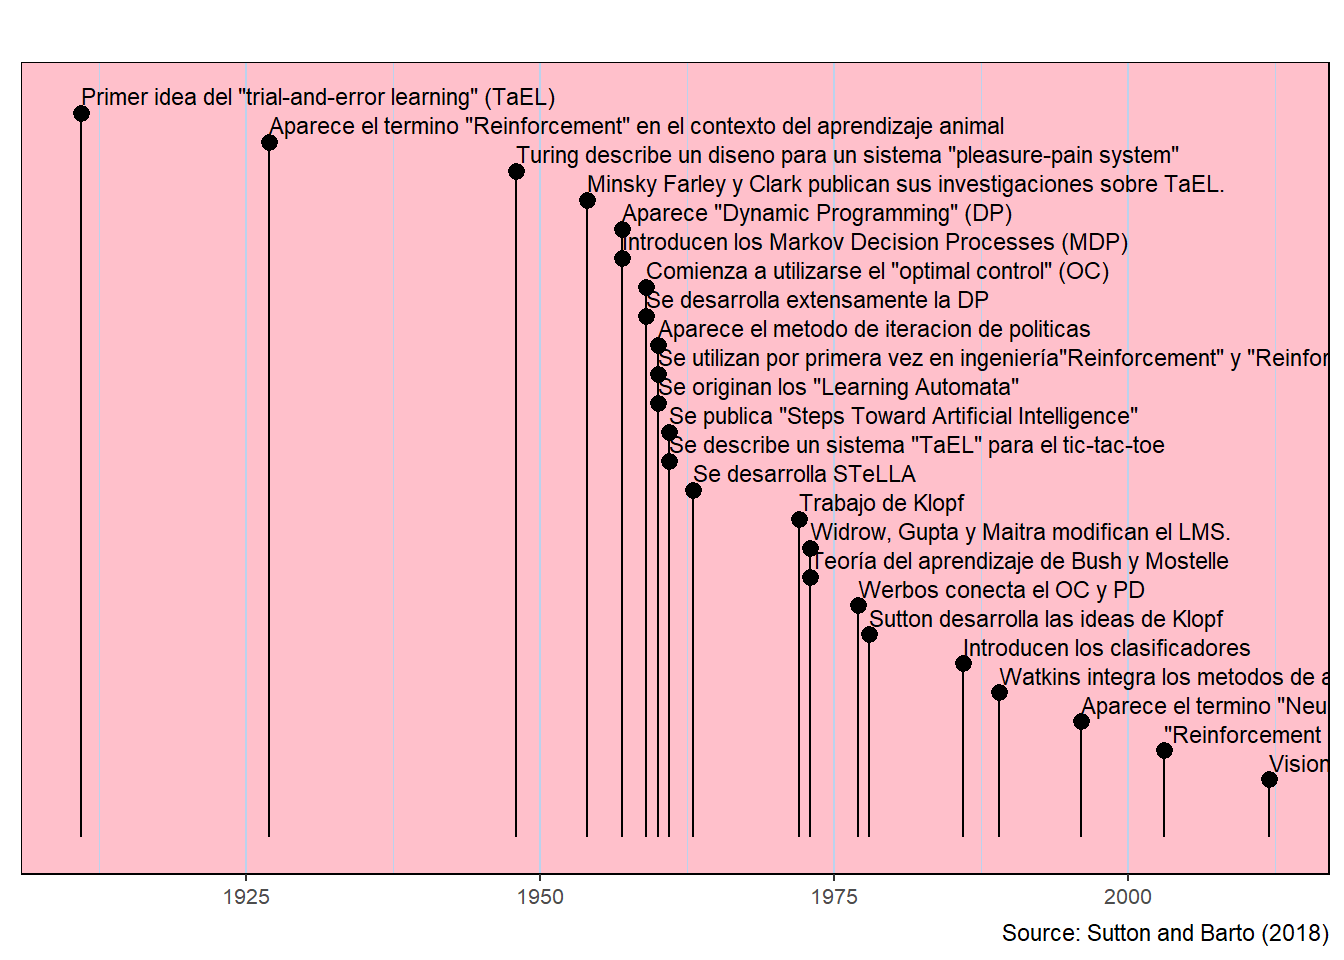
\includegraphics{Tarea-1_files/figure-pdf/unnamed-chunk-4-1.pdf}

\section{EJERCICIO 1}\label{ejercicio-1}

En el aprendizaje reforzado un agente aprende a tomar decisiones
(acciones) a través de la interacción con su entorno y recibiendo
recompensas o castigos en función de las mismas, a diferencia del
aprendizaje supervisado, ya que en este tipo de aprendizaje automático,
un modelo se entrena utilizando un conjunto de datos que incluye tanto
las entradas como las salidas correspondientes (etiquetas). es decir,
consiste en aprender a partir\\
de un conjunto de ejemplos ya etiquetados y proporcionados por un
supervisor externo con conocimientos. Por lo que en este tipo de
aprendizaje Cada ejemplo describe una situación especifica, y además
existe una etiqueta que indica la acción adecuada que el sistema debe
tomar en esa situación, El objetivo de este tipo de aprendizaje es que
el\\
sistema generalice sus respuestas para que actúe correctamente en
situaciones que no están presentes en el conjunto de entrenamiento. Por
otra parte El aprendizaje por refuerzo también es diferente de lo que
los investigadores del aprendizaje automático llaman aprendizaje no
supervisado, que generalmente consiste en\\
encontrar estructuras ocultas en conjuntos de datos no etiquetados y
Aunque en parte el aprendizaje por refuerzo es un tipo de aprendizaje no
supervisado, en realidad este se centra mas que nada en maximizar una
recompensa en lugar de buscar patrones ocultos en los datos.

\section{EJERCICIO 2}\label{ejercicio-2}

es posible pensar que dicha expresión es una función con la cual se mide
el desempeño del sistema bajo diferentes políticas de control dado el
estado inicial, es decir, nos ayuda a identificar que acciones fueron
buenas y cuales fueron malas, además dicha expresión nos da el valor
esperado de cuanta recompensa obtendremos en un futuro al elegir dicha
politica dado un estado inicial. Por otra parte, el factor de descuento
en la expresión, nos ayuda a comparar las recompensas futuras con las
recompensas inmediatas, basicamente nos dice que tan a favor estamos de
obtener una recompensa en el estado actual frente a un futuro lejano

\section{APD}\label{apd}

del algoritmo de la programación dinámica se sigue que para este caso
particular \(J_{N}(x)=\beta^{N}(x_N)^{1-\gamma}\)

luego, para \(k= N-1\)
\[J_{N-1}=\min_{a\in A(x)}\{\beta^{N-1}(a)^{1-\gamma} + \beta^{N}(1+r)^{1-\gamma}(x-a)^{1-\gamma}\}\]
derivando con respecto a \(a\) obtenemos
\[(1-\gamma)\beta^{N-1}a^{-\gamma}- \beta^{N}(1+r)^{1-\gamma}(x-a)^{-\gamma}\]\}
depués igualando a cero
\[(1-\gamma)\beta^{N-1}\[a^{-\gamma}-\beta(1+r)^{1-\gamma}(x-a)^{-\gamma}\]=0\]
entonces \[(\cfrac{x-a}{a})^\gamma=\beta(1+r)^{1-\gamma}\]
\[\cfrac{x-a}{a}=[\beta(1+r)^{1-\gamma}]^{\frac{1}{\gamma}}\]

\bookmarksetup{startatroot}

\chapter{Summary}\label{summary}

In summary, this book has no content whatsoever.

\begin{Shaded}
\begin{Highlighting}[]
\DecValTok{1} \SpecialCharTok{+} \DecValTok{1}
\end{Highlighting}
\end{Shaded}

\begin{verbatim}
[1] 2
\end{verbatim}

\bookmarksetup{startatroot}

\chapter*{References}\label{references}
\addcontentsline{toc}{chapter}{References}

\markboth{References}{References}

\phantomsection\label{refs}
\begin{CSLReferences}{1}{0}
\bibitem[\citeproctext]{ref-knuth84}
Knuth, Donald E. 1984. {``Literate Programming.''} \emph{Comput. J.} 27
(2): 97--111. \url{https://doi.org/10.1093/comjnl/27.2.97}.

\end{CSLReferences}




\end{document}
